\documentclass[11pt,a4paper]{article}

\usepackage[margin=1in]{geometry}
\usepackage{graphicx}
\usepackage{booktabs}
\usepackage{hyperref}
\usepackage{amsmath}
\usepackage{amssymb}
\usepackage{xcolor}
\usepackage{listings}
\usepackage{microtype}
\usepackage{url}
\usepackage{enumitem}
\usepackage{float}

% Page style — workshop-paper compact
\setlength{\parskip}{0.3em}
\setlength{\parindent}{0pt}

\hypersetup{
  colorlinks=true,
  linkcolor=blue!60!black,
  urlcolor=blue!60!black,
  citecolor=blue!60!black,
}

\lstset{
  basicstyle=\ttfamily\small,
  breaklines=true,
  frame=single,
  framesep=4pt,
}

\title{\textbf{nature}: A platform for systematic experimentation\\
       with LLM agent systems}
\author{Chanhyeok Kim\thanks{\texttt{chanhyeok\_kim@icloud.com}}}
\date{\today}

% arXiv submission hint (ignored by non-arXiv LaTeX engines):
% Primary category: cs.SE
% Secondary:        cs.LG
% MSC-class: 68T05 (AI / agents), 68N99 (software)
% ACM-class: I.2.7 (Natural Language Processing), D.2.8 (Software Engineering / Metrics)

\begin{document}
\maketitle

\begin{abstract}
LLM agent systems are production realities whose behavior depends on
many interacting design choices: model, prompt, tool permission,
delegation topology, memory compaction, adapter stack, aggregator
route. Benchmarks that hold the configuration fixed and vary only
the model tell one useful story \textemdash\ they are not the whole
story. This paper presents \textbf{nature}, a platform built to make each
configuration axis a swappable file-based artifact and every run
an event-sourced log that can be replayed, counterfactually forked,
and post-hoc analyzed. Three illustrative studies demonstrate what
the primitives enable: a 5-preset $\times$ 5-task end-to-end
benchmark reveals a 2.3$\times$ cost variance (max/min of per-preset means) and a receptionist
$\times$ downstream-model interaction effect within a single model
family; a component-level probe sweep across 13 local and 11 cloud
models surfaces provider-family qualitative traits and measurement
artifacts (four local models initially mis-scored; one cloud model
unusable via an aggregator's routing layer); and event-pinned
counterfactual forks attribute post-fork metric deltas cleanly to
a single changed lever, a primitive swap-and-run experiments
structurally cannot provide. A 30-fork paired analysis on an
open-ended code-analysis followup shows a 1.38$\times$ Jaccard-CI
tightening ($z=3.19$); the effect's prompt-regime dependence
is characterized across three followup families,
finding it applies cleanly in open-ended analytical regimes
but not in constrained factual or variety-seeking ones. The
platform is open source at
\url{https://github.com/chanhyeok-made/nature-platform}.
\end{abstract}

\section{Introduction}

LLM agent systems have moved from research demos to production
tooling in a short window. Teams shipping them make dozens of
configuration decisions per session: which model drives which role,
how the delegation topology is wired, which tools each role can
call, how memory is compacted, which aggregator routes the calls,
how failures are retried. Every axis interacts with every other.
A researcher-role choice (say, a local phi4:14b vs a cloud
haiku-4.5) is not a model comparison \textemdash\ it is a
multi-host routing decision that shifts the cost/latency frontier
in ways single-model benchmarks cannot detect.

Progress in this space needs a platform where each variable can be
isolated, swapped, and measured \textemdash\ not just an
application framework, not just a static benchmark. \textbf{nature}
is built as one such platform. The contributions:

\begin{enumerate}[leftmargin=*,itemsep=2pt,topsep=2pt]
\item An architecture that treats each configuration axis as a
      first-class, composable, file-based artifact (Pack, Host,
      Agent, Preset).
\item Event-sourced execution that makes every run reproducible,
      post-hoc analyzable, and \emph{uniquely} supports
      event-pinned counterfactuals: forking any recorded session
      at a chosen decision point, continuing under a mutated
      configuration, and attributing the resulting delta cleanly
      to the post-fork variable.
\item Illustrative studies \textemdash\ a 5-preset benchmark
      (\S\ref{sec:preset-benchmark}), a 24-model probe sweep
      (\S\ref{sec:probes}), and two event-pinned ablations
      (\S\ref{sec:ablations}) \textemdash\ that show the platform
      in use and surface findings that single-model benchmarking
      would miss.
\end{enumerate}

\section{Related work}

Group by what each system optimizes for.

\textbf{Application frameworks.} LangChain, LlamaIndex, CrewAI,
and AutoGen are optimized for \emph{building apps} \textemdash\
their primary ergonomics target agent composition and deployment,
not systematic variation across configuration axes. nature is
complementary: its file-based axis decomposition makes each
dimension independently swappable in a way these frameworks do
not directly expose.

\textbf{Production monitoring / evaluation.} LangSmith, Arize,
and Weights \& Biases (prompts) focus on live traces and
pipeline-level eval. They surface per-request data but do not
target isolated-variable experiments: a researcher comparing two
prompts must either run two production traces (confounded by
load-balanced routing and temperature) or set up a separate
offline harness.

\textbf{Static benchmarks.} SWE-bench, AgentBench, HumanEval,
and MLE-bench compare models on fixed task sets. They are
model-axis-fixed by design \textemdash\ the configuration around
the model is assumed away. nature's preset benchmark in
\S\ref{sec:preset-benchmark} shows how much of that assumed-away
space actually moves the metric.

\textbf{Experiment tracking (ML).} MLflow and W\&B track
parameters and metrics but are model-level, not
agent-topology-aware. Event-sourced forks are not a primitive
in any of these.

\textbf{Adjacent: MCP / tool ecosystems.} The MCP spec
standardizes tool-to-model interfaces but does not address
experimentation-over-configuration. nature is layered above it
\textemdash\ MCP can supply tools, nature supplies the experiment
harness around how agents use them.

Gap: \emph{composable, file-based, reproducible experimentation
across every axis of an LLM agent system.} nature's claimed
niche. Table~\ref{tab:related-comparison} maps the gap onto
seven concrete experiment-time capabilities, marked against
representative systems in each category.

\begin{table}[H]
\centering\footnotesize
\setlength{\tabcolsep}{4pt}
\resizebox{\textwidth}{!}{%
\begin{tabular}{l c c c c c c c}
\toprule
Experiment-time capability & LangChain & LangGraph & AutoGen & CrewAI & LangSmith & MLflow/W\&B & nature \\
\midrule
Per-role model swap (single edit)            & $\circ$ & $\circ$ & $\circ$ & $\circ$ & ---     & ---     & $\bullet$ \\
Per-role prompt / tool-permission swap       & $\circ$ & $\circ$ & $\circ$ & $\circ$ & ---     & ---     & $\bullet$ \\
Behavior intervention as composable artifact & ---     & ---     & ---     & ---     & ---     & ---     & $\bullet$ \\
Deterministic replay from session log        & ---     & $\circ$ & ---     & ---     & $\circ$ & ---     & $\bullet$ \\
Mid-execution fork with config mutation      & ---     & $\circ$ & ---     & ---     & ---     & ---     & $\bullet$ \\
Post-hoc metric extraction from log          & ---     & ---     & ---     & ---     & $\bullet$ & $\circ$ & $\bullet$ \\
Component-level isolated capability probes   & ---     & ---     & ---     & ---     & ---     & ---     & $\bullet$ \\
\bottomrule
\end{tabular}}
\caption{Experiment-time capabilities across representative
systems. Marks reflect the system as documented at the time of
this writing, not what is possible with sufficient custom code.
$\bullet$ = repository-native, documented capability exposed as
a first-class experiment primitive (e.g.\ a single declarative
config edit or one named API call). $\circ$ = achievable with
per-experiment custom code (subclassing, manual checkpoint
plumbing, callback wiring) but not exposed as a first-class
primitive. --- = no documented or practical path known.
Bases: LangChain~\cite{langchain}, LangGraph~\cite{langgraph},
AutoGen~\cite{autogen}, CrewAI~\cite{crewai},
LangSmith~\cite{langsmith}, MLflow~\cite{mlflow},
W\&B~\cite{wandb}; LlamaIndex~\cite{llamaindex} is omitted from
the table because its primary axis (data ingestion / retrieval)
sits outside the experiment-axis comparison. The most
load-bearing $\circ$ on the table is LangGraph's
checkpoint primitive: it supports rewind to a prior state, but
resume-under-mutated-configuration (the operation
\S\ref{sec:primitives} formalizes for nature) is not, at the
time of this writing, a documented LangGraph primitive.
LangSmith's $\bullet$ on metric extraction reflects its
trace-based evaluation API; its $\circ$ on replay reflects
trace-inspection support without deterministic re-execution
under modified configuration.}
\label{tab:related-comparison}
\end{table}

\section{Architecture}
\label{sec:architecture}

nature's architecture decomposes an agent system into six
layered artifacts, each of which the paper's case studies vary
as an isolated experimental axis. The decomposition is
deliberately file-based: a contributor authors a new Pack,
Agent, or Preset as a `.json' (schema-validated) plus an
optional `.md' (role instructions), commits the pair to the
repository, and every subsequent run can reference it by name.
No scripting API to learn, no registry to bootstrap.

\textbf{Pack} \textemdash\ interventions (Gate / Listener /
Contributor) bundled as a file-based discoverable unit. A Gate
intercepts tool invocations and can mutate inputs, short-circuit
with synthesized results, or reject. A Listener subscribes to
frame-lifecycle and LLM-span events for passive observation. A
Contributor injects auxiliary content into outgoing LLM
requests. Packs isolate \emph{behavior policy} as a swappable
variable: a change like ``rate-limit expensive tool calls per
frame'' is a single Pack file, not a diff threaded through the
agent loop.

\textbf{Host} \textemdash\ a model endpoint (HTTP base URL +
API-key env var + provider adapter) plus a model catalog.
Decoupled from the role that uses them, so a Preset can reroute
the same role from \texttt{local-ollama::phi4:14b} to
\texttt{anthropic::claude-haiku-4-5} without editing the role
definition. Hosts isolate \emph{model choice} as a swappable
variable.

\textbf{Agent} \textemdash\ role definition (JSON shell + .md
instruction body). The JSON declares allowed tools, the model
reference, and the role description; the .md carries the
prompt. Isolates \emph{prompt / tool permission / role contract}
as a swappable variable. Role variants such as
\texttt{researcher-scout} (path-only) and \texttt{researcher}
(full analysis) share the JSON and differ only in the .md,
enabling the prompt ablation in \S\ref{sec:ablations}.

\textbf{Preset} \textemdash\ declarative composition of Agents
into a team: a `root\_agent', the roster of reachable
sub-agents, `model\_overrides' (per-role Host::model), and
`prompt\_overrides' (per-role instruction-stem swap). Preset
files are the unit at which whole configurations are compared
in \S\ref{sec:preset-benchmark}.

\textbf{Event-sourced frames} \textemdash\ every decision is
appended to a per-session JSONL event log. Frame lifecycle,
LLM requests and responses, tool starts and completions,
delegation boundaries, and compaction events are all events.
Replay is deterministic: \texttt{reconstruct()} rebuilds any
past frame tree from its log without re-invoking LLMs. Metrics
(cost, latency, turn count, tool-error count, sub-frame depth)
are extracted from the log after the fact, not captured at
runtime. This is what makes event-pinned counterfactual forks
possible: a branch copies the prefix log up to event $N$ and
continues from event $N{+}1$ under a new configuration.

\textbf{Memory compaction pipeline} \textemdash\
\texttt{BodyCompactionPipeline} runs before every LLM call,
gated by a per-model context budget. Strategies
(\texttt{MicrocompactBodyStrategy} evicts old tool-results;
\texttt{DreamerBodyStrategy} summarizes and persists the raw
slice to a session-scoped long-term-memory directory) are
swappable \texttt{BodyCompactionStrategy} instances. Every
compaction emits a \texttt{BODY\_COMPACTED} event whose payload
is the post-compaction body snapshot, so replay is byte-
identical. Isolates \emph{context compaction policy} as a
swappable variable.

The six layers compose at session creation: a Preset
references Agents which reference Hosts; Packs install into
the area manager; the Composer consults the compaction
pipeline before each LLM call. A contributor swapping any one
layer does not touch any other.
Figure~\ref{fig:architecture} summarizes the compose-and-dispatch
relationship.

\begin{figure}[H]
  \centering
  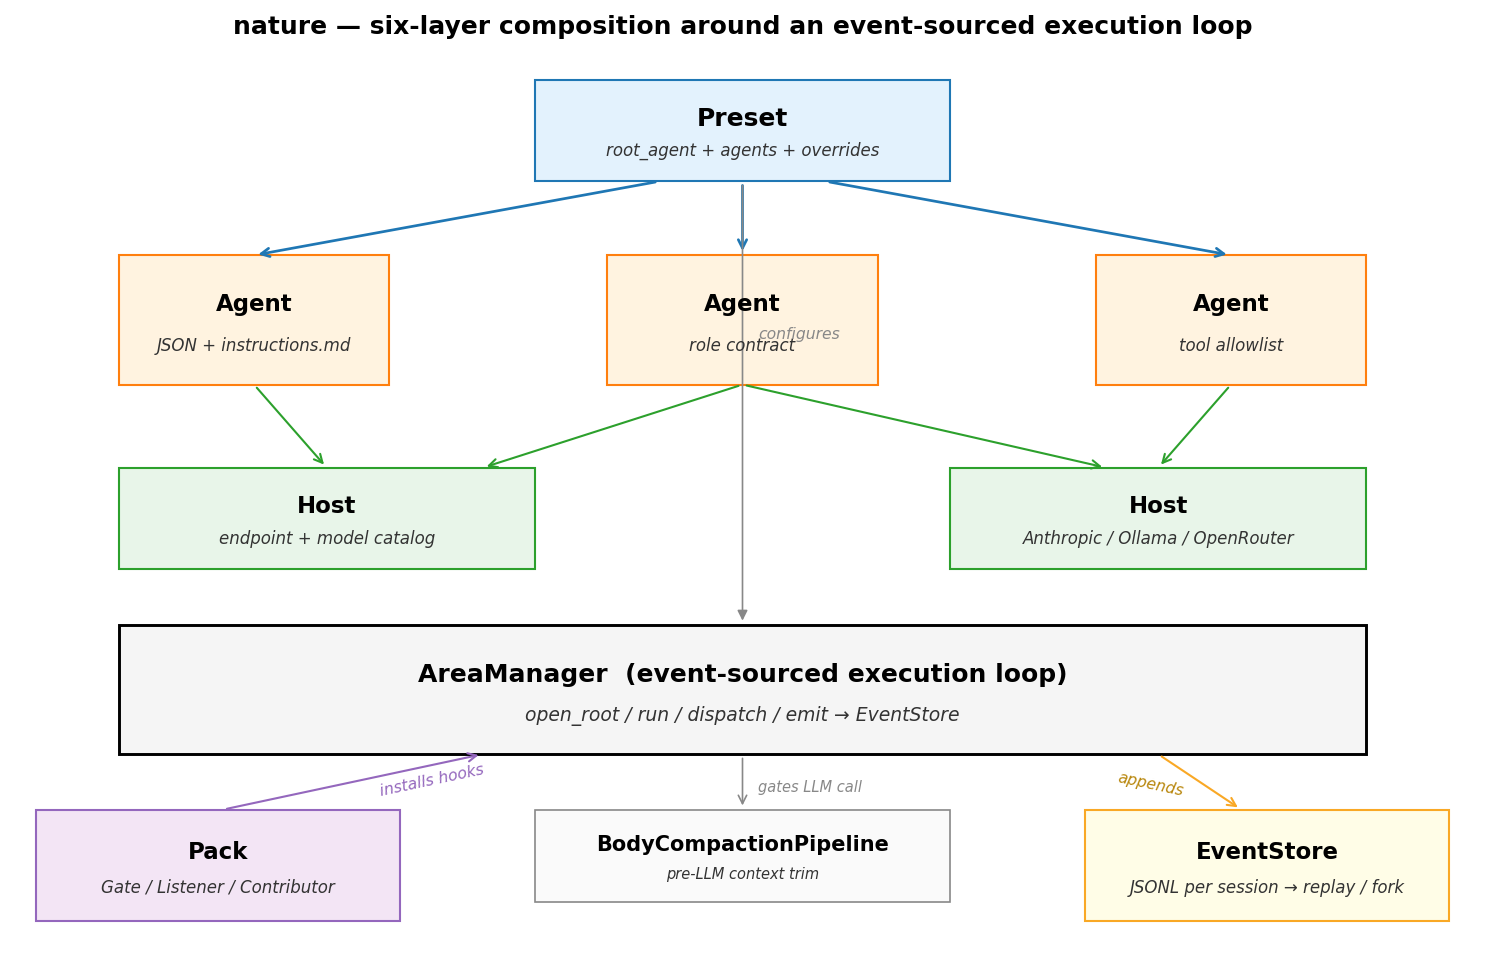
\includegraphics[width=0.95\textwidth]{figures/fig_architecture.png}
  \caption{nature's six-layer architecture. A Preset selects and
           parameterizes Agents; each Agent points to a Host that
           resolves its model; the AreaManager dispatches the
           resulting execution loop and appends every decision to
           the per-session EventStore. Packs install hooks into the
           manager; the BodyCompactionPipeline gates every outgoing
           LLM call. Every edge between layers is a file-based
           artifact reference, not a hard-coded dependency.}
  \label{fig:architecture}
\end{figure}

\section{Experimentation primitives}
\label{sec:primitives}

\textbf{Swap-and-run.} Replace one Pack / Host / Agent / Preset
and re-execute from scratch. Cheap; every source of per-run
variance (sampling, tool state, external call ordering) folds
into the reported delta. Appropriate for broad surveys like
\S\ref{sec:preset-benchmark}.

\textbf{Event-pinned counterfactual divergence.} Because every
decision is an appended event, a recorded session can be
\textbf{forked at any event id}; nature replays the prefix into
a new session and continues from the fork point under a mutated
configuration (different Preset, Host, or Pack set). The
pre-fork state is byte-for-byte shared across branches, so the
post-fork metric delta attributes cleanly to the single variable
that changed. This is the key methodological lever the
event-sourced design unlocks \textemdash\ counterfactuals like
``what if the researcher's model had been swapped at turn 3 of
\emph{this} specific task execution'' become a single API call
rather than a confounded two-session comparison. See
Figure~\ref{fig:fork-schematic} for the schematic and
\S\ref{sec:ablations} for worked examples.

\begin{figure}[H]
  \centering
  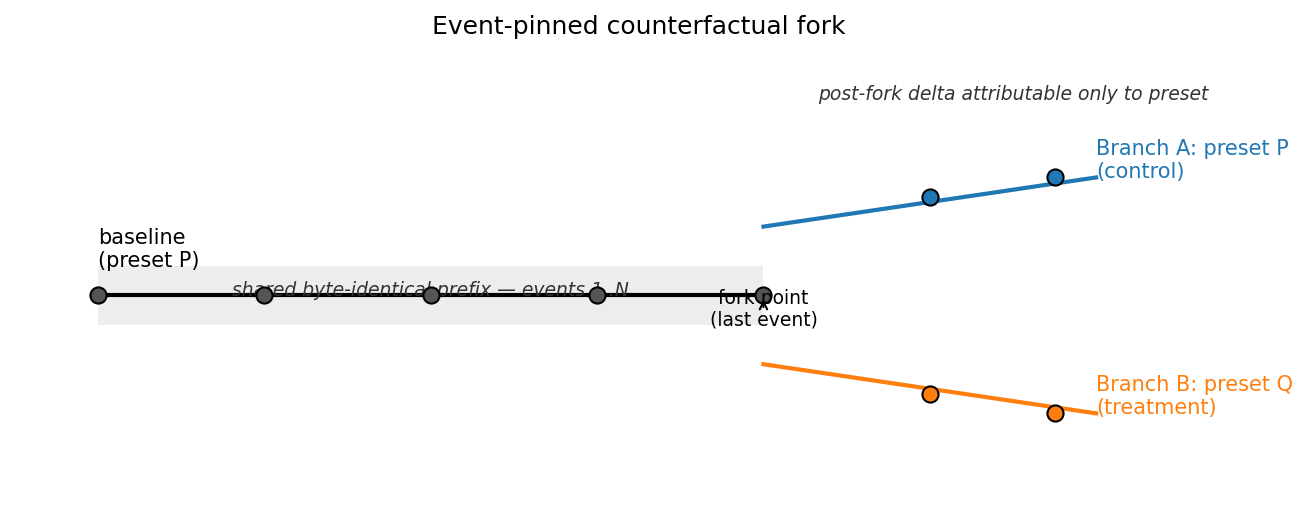
\includegraphics[width=0.88\textwidth]{figures/fig_fork_schematic.png}
  \caption{Event-pinned counterfactual fork schematic.
           Branches inherit a byte-identical prefix and diverge
           only in the post-fork configuration.}
  \label{fig:fork-schematic}
\end{figure}

\textbf{Formal definition.} A nature session $s$ is a pair
$(E_s, c_s)$ where $E_s = (e_1, \ldots, e_n)$ is its append-only
event log and $c_s$ is its resolved configuration (agent roster,
per-role model overrides, Pack installations, prompt overrides).
The event log is the sole source of truth for replay. The fork
operation is
$$
  \mathrm{fork}(s, k, c') \to s', \qquad 1 \le k \le |E_s|,
$$
producing a session $s' = (E_{s'}, c')$ with
$E_{s'}[1{:}k] = E_s[1{:}k]$ (byte-identical prefix); subsequent
events $e_{k+1}^{s'}, e_{k+2}^{s'}, \ldots$ are generated under
$c'$. Two confounds the operation eliminates: (i) any metric
defined over the shared prefix is identical between $s$ and $s'$
by construction, and (ii) any post-fork metric difference between
two siblings $s_A = \mathrm{fork}(s, k, c_A)$ and
$s_B = \mathrm{fork}(s, k, c_B)$ attributes to the configuration
delta $c_A \mathbin{\ominus} c_B$ rather than to pre-fork
stochasticity. The remaining post-fork variance is limited to
exogenous and runtime nondeterminism that occurs after the fork
point: LLM sampling, tool-call side effects, external API or
file-state drift between the two sibling runs, aggregator-level
routing instability, and runtime scheduling artifacts. The
operation does not eliminate this remaining noise; it isolates
the pre-fork prefix as a controlled constant. For paired analysis
the same $(s, k)$ is forked twice with $c_A$ and $c_B$, yielding
paired observations whose covariance via the shared prefix
tightens the standard error of the metric difference (next
paragraph).

\textbf{Paired analysis via fork.} Two branches forked from the
same baseline yield paired observations per baseline, so the
standard error of the metric difference is
$\mathrm{Var}[B-A] = \mathrm{Var}[A] + \mathrm{Var}[B] - 2\,\mathrm{Cov}[A,B]$
rather than the unpaired
$\mathrm{Var}[A]/n_A + \mathrm{Var}[B]/n_B$. The covariance
term is the statistical lever: baseline content that transmits
into both branches' post-fork responses yields
$\mathrm{Cov}[A,B] > 0$ and a tighter paired CI. This is
verified empirically at $N=30$ paired trials on a short
code-analysis followup (\texttt{direct-core} baseline $\to$
A=\texttt{direct-core} vs B=\texttt{haiku-phi4}):

\begin{table}[H]
\centering\small
\begin{tabular}{l r r r}
\toprule
metric & unpaired 95\,\% CI halfwidth & paired & ratio \\
\midrule
response length (chars) & 41.1 & 31.2 & 1.32 \\
Jaccard token overlap   & 0.091 (unpaired mean) & 0.126 (paired mean) & 1.38 ($z=3.19$) \\
\bottomrule
\end{tabular}
\end{table}

Both metrics show paired tightening; the Jaccard ratio is
slightly larger, consistent with content-linked metrics
inheriting more baseline covariance than surface metrics.

\textbf{Why token Jaccard?} Token-set Jaccard is chosen over
embedding-cosine and exact-match alternatives for three reasons.
First, it is deterministic and provider-independent: there is no
reliance on a specific embedding model whose output drifts across
versions, and replication of the analysis requires only the
recorded text and a stop-word list. Second, it is bounded $[0,1]$
and symmetric, which makes the per-baseline paired/unpaired ratio
a well-formed statistic; the ratio is also robust to template
words that appear in both branches because such words contribute
identically to paired and unpaired comparisons and cancel.
Third, on the paper's prompts (open-ended analytical, factual
diff, code summarization) the relevant question is not paraphrase
equivalence but whether the post-fork branches \emph{name the
same architectural concepts} (e.g.\ ``EventStore'', ``cascade
depth'', ``WebSocket reconnection''); token overlap captures this
directly, while embedding cosine would also reward fluent
paraphrases that mention nothing concrete in common. The cost is
real: Jaccard ignores semantic equivalence ($J(\{x_1\}, \{y_1\})
= 0$ even when $x_1$ and $y_1$ are synonyms) and is sensitive to
the stop-word list. A semantic-similarity replication is a
natural future check.

\textbf{Regime conditioning.} The tightening is \emph{not} a
universal property of event-pinned forks. The test was extended
to three prompt regimes ($n=15$ each, same A/B branch
structure): P1 asks the model to identify ONE concrete risk
from a prior code analysis (\emph{open-ended analytical}); P2
asks for ONE runtime consequence of a noted preset difference
(\emph{constrained factual}); P3 asks for ONE potential
failure mode in a module just summarized (\emph{selection
with variety pressure}). Only P1 shows a significant paired
tightening (Figure~\ref{fig:paired-regime}):

\begin{table}[H]
\centering\small
\begin{tabular}{l r r r}
\toprule
prompt regime & paired Jaccard & unpaired & ratio ($z$) \\
\midrule
P1 open-ended analytical       & 0.170 & 0.100 & 1.71 ($z=3.41$) \\
P2 constrained factual         & 0.197 & 0.187 & 1.05 ($z=0.70$) \\
P3 selection, variety-sought   & 0.122 & 0.127 & 0.96 ($z=-0.28$) \\
\bottomrule
\end{tabular}
\end{table}

\begin{figure}[H]
  \centering
  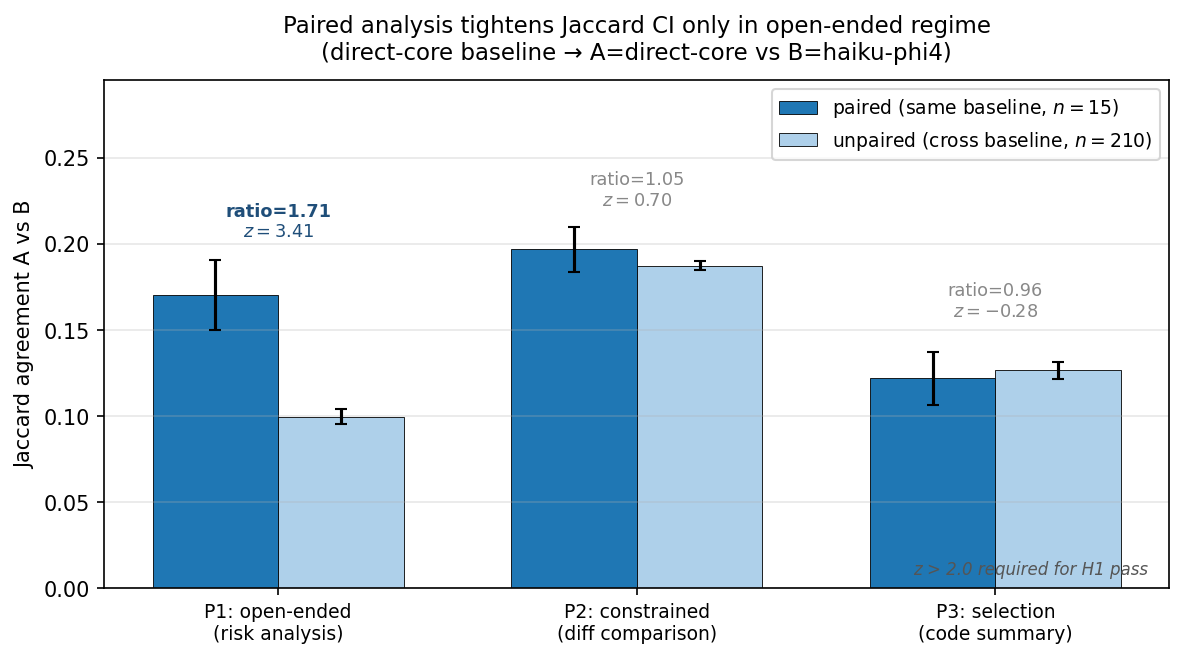
\includegraphics[width=0.88\textwidth]{figures/fig_paired_jaccard_regime.png}
  \caption{Paired vs unpaired Jaccard across three prompt
           regimes ($n=15$ per regime,
           \texttt{direct-core}$\to$\texttt{haiku-phi4} fork).
           Only the open-ended analytical regime shows
           significant CI tightening; factual and
           selection-with-variety regimes do not benefit.
           Paired bars show same-baseline A--B agreement;
           unpaired bars pool cross-baseline comparisons.}
  \label{fig:paired-regime}
\end{figure}

Interpretation: paired analysis tightens CI when baseline
content \emph{steers} the followup answer choice. Prompts
where the factual answer is already determined (P2) or where
the followup is expected to diversify across seeds (P3) fall
outside this regime. Practitioners using fork's paired
structure should pilot with small $n$ before committing; the
CI reduction is contingent, not guaranteed.

\textbf{Replay with modification.} \texttt{reconstruct()}
rebuilds any past frame tree from its jsonl log \textemdash\ for
post-hoc metric extraction, tool behavior analysis, regression
testing of framework-level changes against an archive.

\textbf{Shareable artifacts.} Pack, Agent, Preset, Host, task,
and probe definitions are file-based with strict schemas.
Experiments and their results can be version-controlled and
shared verbatim.

\textbf{Probes.} JSON-defined single-axis capability tests
(tiered T0\textendash T9, \S\ref{sec:probes}) that isolate one
dimension (\texttt{tool.emit}, \texttt{edit.discipline},
\texttt{multi\_turn\_state}, etc.) with structural success
criteria. Composable with Host + Preset the same way
\texttt{nature eval} is.

\section{Case study: preset-level benchmark}
\label{sec:preset-benchmark}

\subsection{Setup}

Five presets span two binary design axes (receptionist vs
no-receptionist topology; cloud-only vs hybrid downstream
model class), producing a 2$\times$2 factorial of cloud / hybrid
configurations, plus a fifth all-local configuration. They run
against five tasks covering three setup types and one
acceptance method (pytest).

\begin{table}[H]
\centering\small
\begin{tabular}{l c c c c c c c}
\toprule
preset & recep. & core & research. & analyz. & impl. & review. & judge \\
\midrule
\texttt{default}              & H & S & H & S & S & H & H \\
\texttt{direct-core}          & -- & S & H & S & S & H & H \\
\texttt{haiku-phi4}           & H & H & H & P & H & P & P \\
\texttt{direct-haiku-phi4}    & -- & H & H & P & H & P & P \\
\texttt{local-role-optimized} & -- & Q & P & Q & Q & P & P \\
\bottomrule
\end{tabular}
\end{table}

\textit{Legend:} H=\texttt{claude-haiku-4-5}, S=\texttt{claude-sonnet-4-6}
(Anthropic API); P=\texttt{phi4:14b}, Q=\texttt{qwen2.5:72b}
(both Ollama-hosted, Q4\_K\_M quantization). An em-dash (\texttt{--})
means the role is omitted from the preset's roster (no receptionist
layer in \texttt{direct-*} presets). The 2.3$\times$ cost variance
within the four cloud presets (max/min of per-preset cost means
across passed cells; \S\ref{sec:preset-benchmark} results) is
driven by (a)~\texttt{direct-core} / \texttt{default} routing
core/analyzer/implementer to Sonnet and (b)~\texttt{haiku-phi4} /
\texttt{direct-haiku-phi4} restricting cloud roles to Haiku while
offloading analyzer/reviewer/judge to local phi4.

\textbf{Experimental setup.} Hardware: Mac Studio, Apple M2 Max,
96\,GB unified memory. Local inference: Ollama 0.20.5 at Q4\_K\_M.
Cloud inference: Anthropic direct API (no aggregator). All agents
use their per-agent default temperature; no preset-level overrides.
nature CLI 0.3.0. All preset and agent JSON files plus task
definitions are in the paper's accompanying repository at
\url{https://github.com/chanhyeok-made/nature-platform}.

Tasks: \texttt{s1-csv-parser} (small patch, pytest),
\texttt{s3-json-pointer} (small patch, pytest),
\texttt{s4-async-refactor} (medium refactor, pytest),
\texttt{n1-pack-discovery} (medium feature, pytest),
\texttt{x1-pluggy-remove-plugin} (external repo, pytest). Each
cell runs 2 seeds under a 600\,s session watchdog.

\subsection{Results}

\begin{figure}[H]
  \centering
  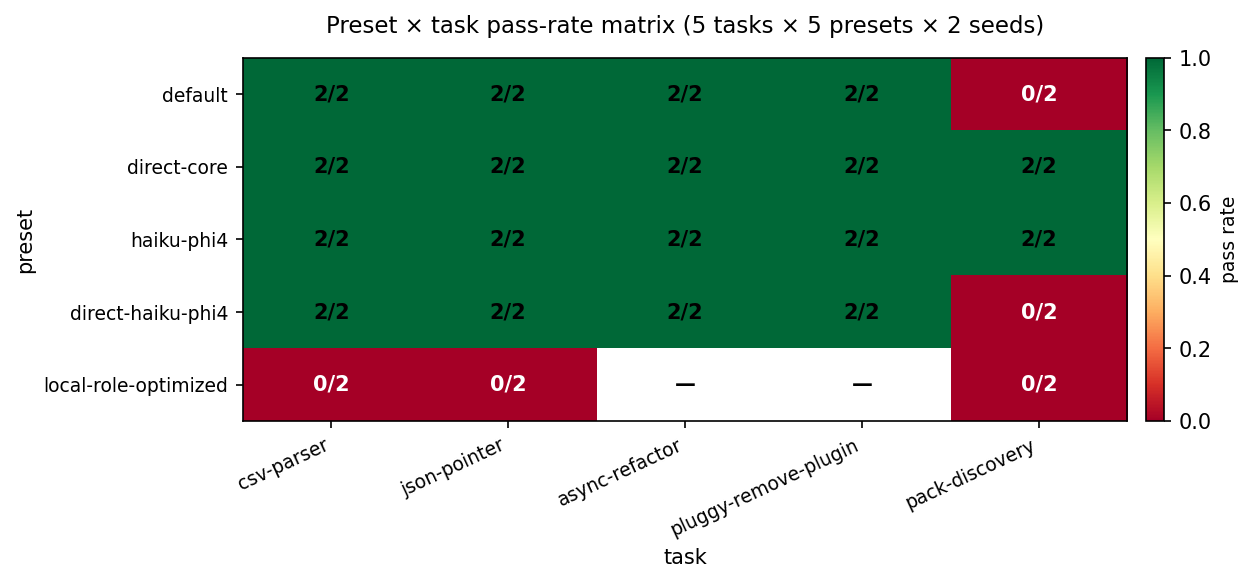
\includegraphics[width=0.95\textwidth]{figures/fig_preset_task_heatmap.png}
  \caption{Pass-rate matrix across 5 presets and 5 tasks. Cells
           are $\{$0, 1, 2$\}$ / 2; color encodes rate, numbers
           show $k/n$. \texttt{local-role-optimized} ran on three
           tasks only (all 0/2).}
  \label{fig:heatmap}
\end{figure}

Figure~\ref{fig:heatmap} summarizes pass rates. Three findings:

\begin{enumerate}[leftmargin=*,itemsep=2pt,topsep=2pt]
\item \textbf{Only \texttt{n1-pack-discovery} discriminates
      among cloud/hybrid presets.} On the other four tasks, every
      non-local preset passes both seeds. The entire
      configuration-sensitivity signal among
      \texttt{default} / \texttt{direct-core} /
      \texttt{haiku-phi4} / \texttt{direct-haiku-phi4} is driven
      by their different behavior on n1.
\item \textbf{\texttt{local-role-optimized} does not pass.} Five
      of six cells timed out at 600\,s; the sixth ran to
      acceptance and failed at pytest. Turn counts 6\textendash 17,
      tool-error counts 0\textendash 7 \textemdash\ the model was
      emitting ill-formed tool arguments faster than it made
      progress.
\item \textbf{The 2$\times$2 factorial} of the other four
      presets (Figure~\ref{fig:factorial}) suggests the
      receptionist layer helps on the hybrid (100\,\% vs
      80\,\%) but hurts on pure-haiku (80\,\% vs 100\,\%).
      An interaction-consistent crossed-paths pattern is
      visible in the four observed cells; the per-cell $n=2$
      precludes a hypothesis test on the interaction itself
      (see \S\ref{sec:limitations}'s sample-size note), so
      this is reported as an observed pattern, not a
      statistically established effect.
\end{enumerate}

\begin{figure}[H]
  \centering
  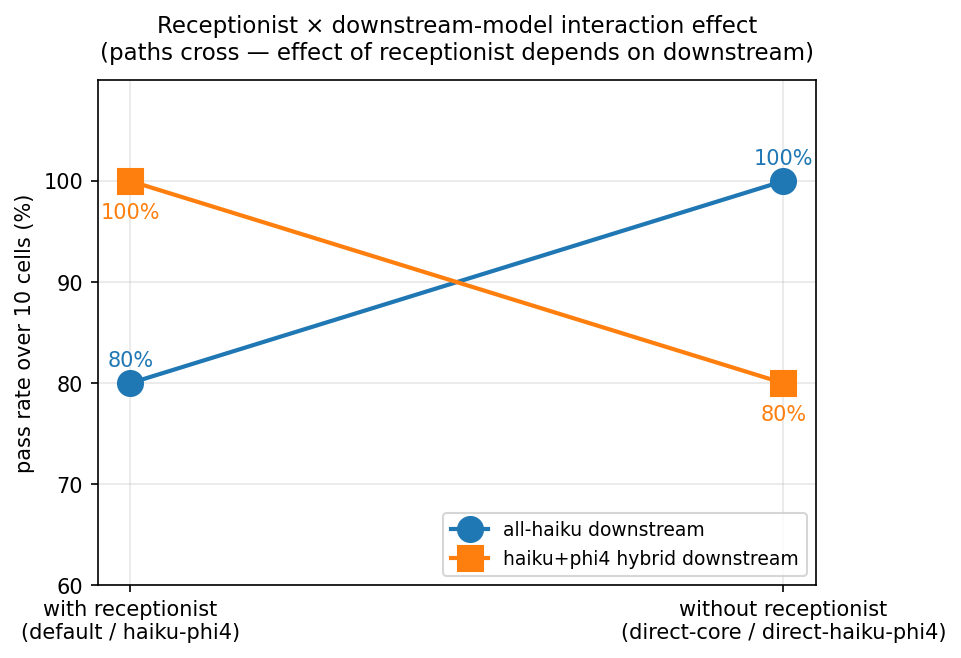
\includegraphics[width=0.75\textwidth]{figures/fig_factorial_interaction.png}
  \caption{Receptionist $\times$ downstream-model interaction.
           Adding a receptionist helps hybrid downstream but
           hurts all-haiku downstream.}
  \label{fig:factorial}
\end{figure}

\begin{figure}[H]
  \centering
  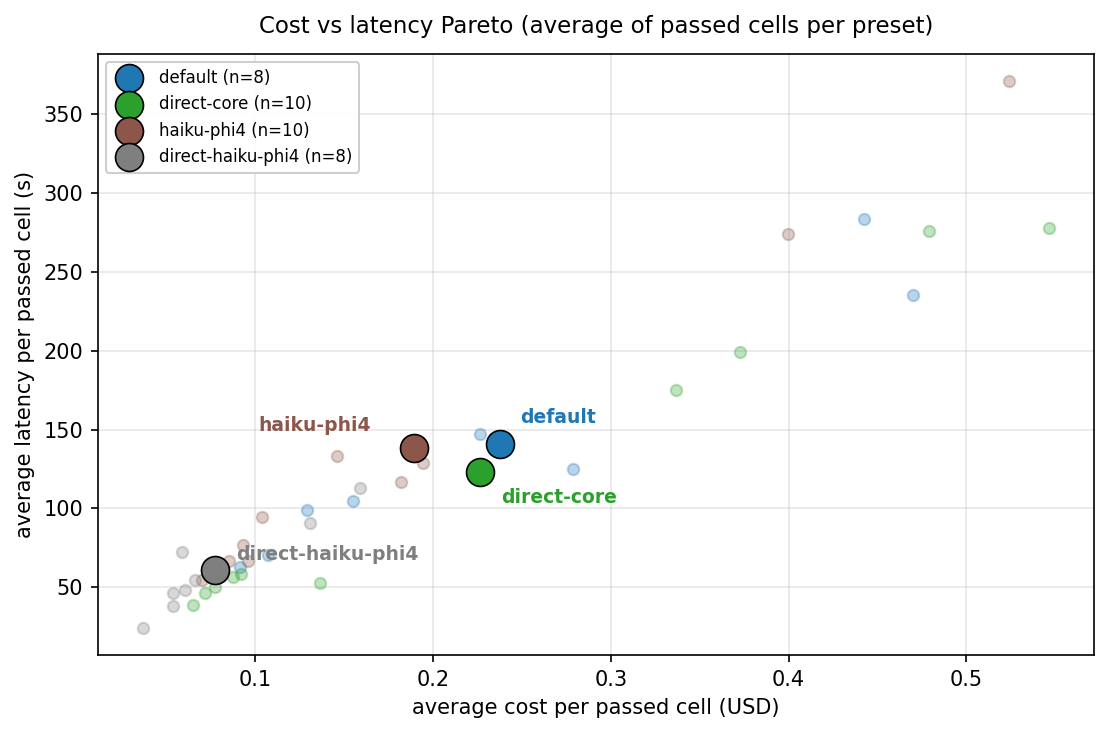
\includegraphics[width=0.85\textwidth]{figures/fig_cost_latency_pareto.png}
  \caption{Cost vs latency across presets (means over passed
           cells). \texttt{haiku-phi4} and \texttt{direct-core}
           are Pareto-competitive; \texttt{direct-haiku-phi4}
           is cheapest and fastest but carries silent-failure
           risk on n1.}
  \label{fig:pareto}
\end{figure}

\begin{figure}[H]
  \centering
  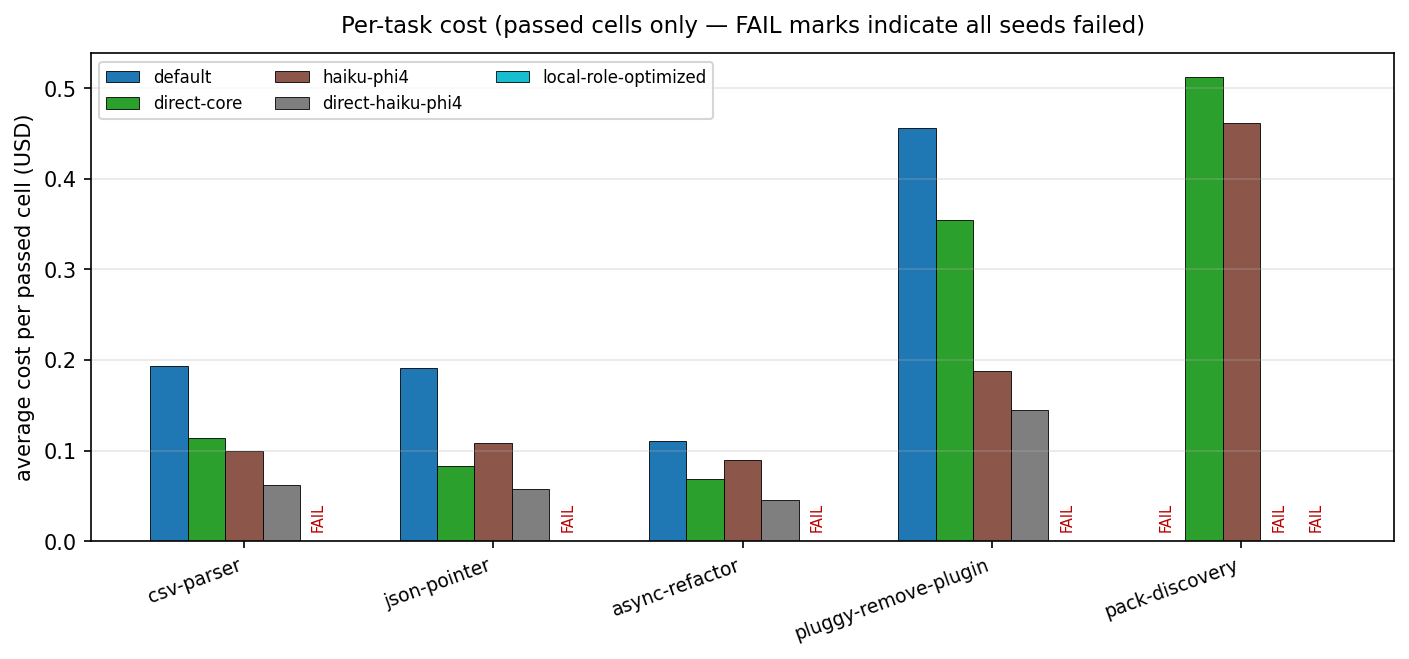
\includegraphics[width=0.95\textwidth]{figures/fig_per_task_cost.png}
  \caption{Per-task cost on passed cells only. ``FAIL'' marks
           indicate all seeds of that cell failed.}
  \label{fig:per-task-cost}
\end{figure}

\subsection{A trace-based hypothesis for the observed pattern}

Event log audit of the four failing and two narrowly-passing n1
cells yields a candidate causal story (offered as a
trace-grounded hypothesis, not a tested mechanism). \texttt{default} on n1 averaged 91
turns at timeout with 124 tool calls and 13 tool errors
\textemdash\ a receptionist $\to$ core $\to$ 4-sub-agent loop that
spawned 14\textendash 18 sub-frames per session without resolving.
\texttt{direct-core} on the same n1 passed both seeds at 38 turns
average and 7\textendash 8 sub-frames: the absent receptionist
meant core planned from the user's original prompt directly and
the researcher delegation was cleaner.

On the hybrid, the pattern flipped. \texttt{haiku-phi4} passed
n1 despite 12\textendash 15 tool errors per session
\textemdash\ \emph{more errors than \texttt{default}}
\textemdash\ because the receptionist layer acted as redundant
supervision that caught phi4's formatting mistakes. Stripping
the receptionist (\texttt{direct-haiku-phi4}) produced faster
completion (173\textendash 248\,s) but with a silent
\emph{wrong answer}: pytest failed on
\texttt{test\_install\_entry\_can\_reach\_neighbouring\_modules}.
The receptionist acted as insurance that pays premium when the
downstream is strong and pays dividends when the downstream is
weak.

\subsection{Sample-size caveat}

Per-cell $n=2$. Wilson 95\,\% CI for 10/10 is [72.2\,\%, 100\,\%];
for 8/10 is [49.0\,\%, 94.3\,\%]. The intervals overlap. No
claim of statistical significance is made on pass-rate
differences between close presets \textemdash\ the evidence is
trace-level (turn count, sub-frame structure, cost-by-agent,
error signatures) rather than hypothesis-test. For stronger claims the
matrix needs 5\textendash 10 seeds per cell and more tasks
(\S\ref{sec:limitations}).

\section{Case study: component-level probes}
\label{sec:probes}

Preset-level benchmarks answer ``which configuration completes
this task'' but leave the \emph{why} opaque. A
\texttt{(host, model)} that fails on one preset and succeeds on
another might have a wrong prompt, a wrong tool, a wrong model
choice, or a latent infrastructure bug. A \emph{probe} suite was
designed: 32 tier-graded capability tests each
isolating one axis (tool-use, edit-discipline, multi-turn state,
etc.) with structural pass/fail criteria, so runs are
deterministic and replayable. Probes are first-class nature
artifacts and compose with the Host + model layer the same way
\texttt{nature eval} does. Full per-probe discussion is in the
paper repository; headline findings appear below.

\subsection{Local sweep: 13 Ollama-hosted models}

Every model in the first probe pass produced scores later
determined to be substantially inflated or deflated by latent
infrastructure bugs. Four cases (phi4:14b 3\textendash 25,
qwen2.5-coder:32b 4\textendash 21, llama3.3:70b 3\textendash 22,
command-r7b unchanged post-fix) each mapped to a specific bug in
the adapter/wrapper/timeout stack; each repair shifted the
apparent model ranking. The lesson: \emph{infrastructure
configuration is a measurement variable}. Benchmark reports that
do not disclose the adapter stack they ran under are incomplete.

\subsection{Cloud sweep: 11 OpenRouter-routed models}

Eleven cloud models via OpenRouter $\times$ 32 probes
(+ 12 borderline probes re-run at 2 additional seeds) produced
$\approx$616 cells at total spend \$2.56. Headline findings:

\begin{itemize}[leftmargin=*,itemsep=2pt,topsep=2pt]
\item \textbf{Universal long-context ceiling.} \texttt{t3-32k}
      and \texttt{t4-128k} (needle-in-haystack over repetitive
      content) fail 11/11. Needle retrieval from repetitive
      long-context is the current cloud ceiling shared across
      providers and generations.
\item \textbf{Provider-family qualitative traits.} Gemini
      family (flash + pro) consistently paraphrases verbatim
      instructions (\texttt{activeForm} field); Mixtral 8$\times$22B
      fabricates single characters in long random-looking temp
      paths; gpt-4o chose \texttt{limit=1} on a paginated Read
      and declared the file empty after two turns; llama-3.3-70B
      produced the highest schema-adherence instability (9/12
      borderline probes non-consistent-pass across 3 seeds: 8
      flaky plus 1 consistent-fail). None of these
      surface on a single-host measurement.
\item \textbf{Platform friction as measurement variable.}
      \texttt{qwen-2.5-coder-32b} is listed in the OpenRouter
      catalogue but routes to Cloudflare Workers AI, which
      (a) advertises no tool-use endpoint (HTTP 404) and
      (b) returns mid-stream 500s on trivial text prompts. The
      same open-weight model works fine via local Ollama.
\end{itemize}

\subsection{Contrast}

On the shared 29-probe subset, 10 cloud models cluster at
25\textendash 29/29 (4-point spread across 10 models); 13 local
models span 2\textendash 25/29 (23-point spread). Best local
(\texttt{phi4:14b}, \texttt{qwen2.5:72b}) meets worst cloud
(\texttt{llama-3.3-70b} via OpenRouter) at 25/29. Two models
appear in both surveys; cloud adds 2\textendash 3 passes out of
29 over local q4\_K\_M of the same weights
\textemdash\ attributable to higher effective precision plus
escape from consumer-hardware first-token latency.

\textbf{Connection to the workflow demonstration.} The probe
ranking serves as an empirical prior for the fork-based tuning
workflow of \S\ref{sec:ablations}: candidates for a given role
are pre-screened on dimensions that role exercises (e.g.\
\texttt{tool.emit}, \texttt{edit.discipline}, \texttt{multi\_turn\_state}
for analyzer/reviewer roles), and only the top probe-tier
candidates are forked into the live session for paired
verification. The 25/29 score for \texttt{phi4:14b} is what
motivates its selection as the analyzer/reviewer/judge swap
candidate in \S\ref{sec:ablations}'s model-swap ablation; the
fork primitive then verifies whether that probe-level capability
translates to baseline-consistent post-fork behavior on a real
session. Without §\ref{sec:probes}'s prior, \S\ref{sec:ablations}
would be exploring an unscoped candidate space; without
\S\ref{sec:ablations}'s in-session verification, \S\ref{sec:probes}'s
probe scores would be untested as routing recommendations.

\section{Illustrative ablations}
\label{sec:ablations}

Two event-pinned ablations demonstrate the fork primitive.

\subsection{Prompt ablation}

Baseline: \texttt{direct-core} preset on a focused
code-analysis prompt. After completion (34 events), the session
was forked at its last event into two branches that received an
identical follow-up prompt:

\begin{itemize}[leftmargin=*,itemsep=2pt,topsep=2pt]
\item Branch A (control): \texttt{direct-core} with default
      \texttt{researcher.md} (broad mode).
\item Branch B (treatment): \texttt{direct-core-scout} with the
      researcher role's instruction stem overridden to
      \texttt{researcher-scout}, which returns \emph{only} file
      paths, no contents.
\end{itemize}

Both branches identified the same high-level architectural risk
(parallel delegation with no concurrency cap). Branch A's
researcher returned file contents; Branch B's scout returned
only paths, and core synthesized the risk from path semantics +
structural inference. Scope-restricted sub-agent prompts did not
prevent the caller from arriving at the same architectural
observation \textemdash\ a useful data point for cost/latency
optimization, and one that a swap-and-run comparison could not
make precise because fresh-run baselines diverge from event 1.

\subsection{Model-swap ablation ($n=15$ seeds)}

Fifteen independent \texttt{direct-core} baselines, each forked
at its last event into a control branch (\texttt{direct-core})
and a treatment branch (\texttt{haiku-phi4}:
analyzer/reviewer/judge replaced with phi4:14b local). All
thirty branches received the same P1 open-ended followup
(identify ONE concrete risk in the architecture just
described, 2--3 sentences). This is the event-pinned
demonstration of \S\ref{sec:primitives}'s fork primitive
operating in the regime where paired analysis is expected to
help; the candidate model (phi4:14b) was selected from
\S\ref{sec:probes}'s local sweep (25/29 probe pass,
local-top tier) as a probe-informed prior for the
analyzer/reviewer/judge roles.

\begin{figure}[H]
  \centering
  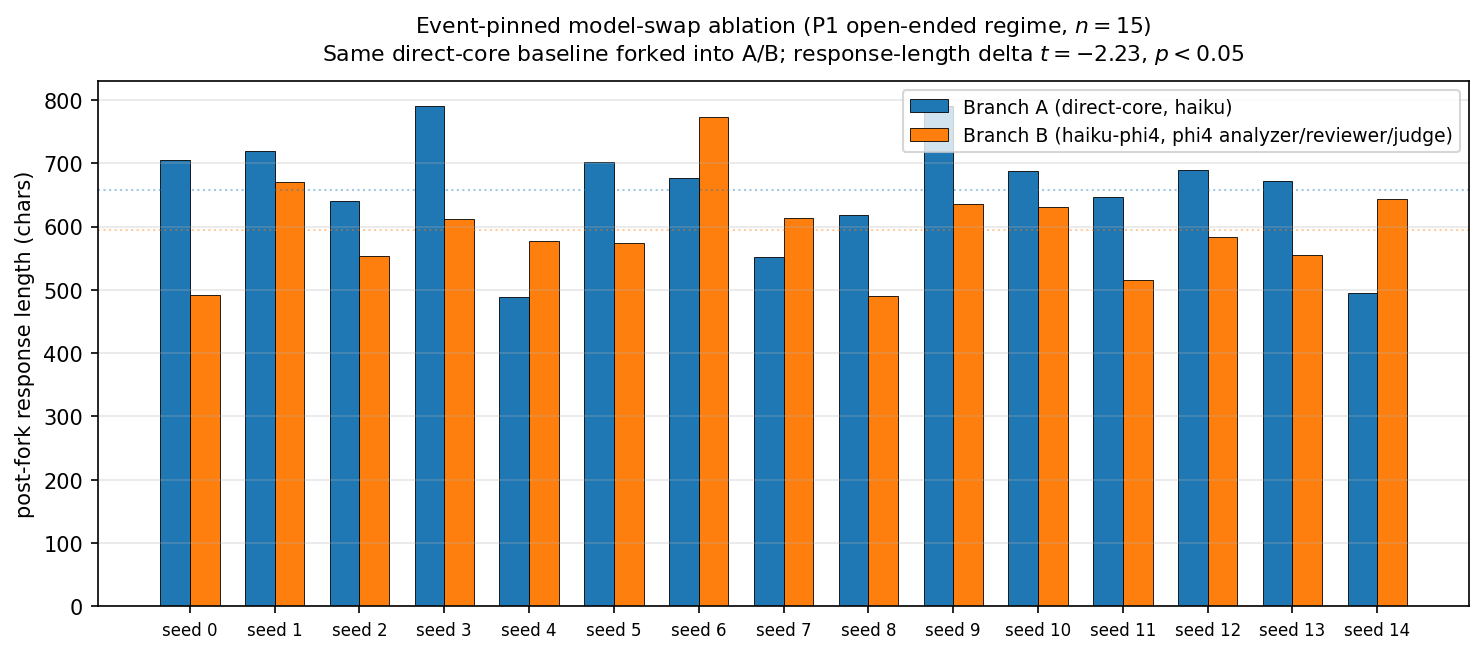
\includegraphics[width=0.92\textwidth]{figures/fig_ablation_model_swap.png}
  \caption{Event-pinned model-swap ablation ($n=15$ paired
           seeds, P1 open-ended regime). Each seed's
           \texttt{direct-core} baseline is forked into A
           (\texttt{direct-core}, control) and B
           (\texttt{haiku-phi4}, treatment) with byte-identical
           prefix. Mean lines dashed. Paired $t=-2.23$
           ($p<0.05$) on response length.}
  \label{fig:ablation}
\end{figure}

Three findings:

\begin{itemize}[leftmargin=*,itemsep=2pt,topsep=2pt]
\item \textbf{Paired Jaccard tightens CI at $z=3.41$.}
      Same-baseline A--B token overlap averages 0.170;
      cross-baseline averages 0.100 (ratio 1.71,
      Figure~\ref{fig:paired-regime}). The post-fork delta
      is attributable to the subagent model swap; cross-seed
      stochasticity is controlled by pairing. This is the
      empirical payoff of the primitive of
      \S\ref{sec:primitives}.
\item \textbf{Branch B runs shorter by $64 \pm 29$ chars.}
      Phi4 local analyzer/reviewer/judge produces terser
      final responses than haiku (paired $t=-2.23$,
      $p<0.05$). In ancillary measurements across the three
      prompt regimes of \S\ref{sec:primitives}, the verbosity
      reduction persists: P2 $-129 \pm 21$ ch ($t=-6.03$,
      $p<0.001$), P3 $-77 \pm 24$ ch ($t=-3.17$, $p<0.01$).
      The $\sim$10--25\,\% brevity is orthogonal to the
      analytical content agreement captured by paired Jaccard
      and is a separate practical observation: phi4 as a
      subagent is a capacity/verbosity tradeoff point
      independent of its pass/fail probe tier.
\item \textbf{Qualitative convergence and divergence both
      occur.} In some seeds the branches converge on the
      same concrete risk (e.g.\ seed~0: both branches
      identify \texttt{AreaManager} as a god object with
      1504 lines; other seeds: both land on EventStore as
      SPOF or on parallel-tool race conditions). In other
      seeds they reach related-but-distinct risks. The
      paired Jaccard captures this at aggregate; no single
      seed is load-bearing.
\end{itemize}

Reading this as one workflow step under
\S\ref{sec:primitives}: probe data identified phi4:14b as a
local-top candidate; the event-pinned fork confirmed the
post-fork direction stays baseline-consistent (paired Jaccard
1.71 at $z=3.41$); verbosity dropped $\sim$10\,\% without
loss of analytical substance. A practitioner working in
P1-style workloads can \emph{accept} this swap. The same
decision for P2/P3-style workloads would require a separate
fork probe, since paired analysis does not apply there
(\S\ref{sec:primitives}).

\section{Discussion}
\label{sec:discussion}

\textbf{What the case studies do not claim.} Three
generalizations are deliberately refused: no winning preset (on
\S\ref{sec:preset-benchmark}'s task distribution some
configurations tie at 10/10 and could rank differently on a
different distribution), no model ranking (probe rankings depend
on the adapter stack), and no statistical significance (per-cell
$n = 2$ is not enough for pass-rate hypothesis tests).
Comparative claims are grounded in trace-level evidence, not raw
pass-rate deltas.

\textbf{Implications for practitioners.} A reader arriving from
the ``which model should I use'' question should leave asking
``which configuration, given my cost budget and latency tolerance,
on my task distribution.'' The four cloud presets in
\S\ref{sec:preset-benchmark} all use the same frontier model
family and produce 80\textendash 100\,\% pass rates with
2.3$\times$ cost and 1.5$\times$ latency ranges (per-preset means).
Selecting the best
configuration is worth more than swapping the model within-tier.

\textbf{Implications for research.} File-based artifacts
(Pack, Preset, Agent, Probe, task) are readable, diff-able,
git-tractable. A new Probe or Task is a markdown plus a JSON
schema, nothing more. This is treated as an experiment in
whether community contribution of agent-system components can be
as lightweight as contributing a benchmark task to a research
repository. Event-sourced forks are the primitive not yet
found in prior systems; \S\ref{sec:ablations} argues they are
the right tool for configuration-variance research when the
change point is mid-execution rather than at $t=0$.

\section{Limitations and future work}
\label{sec:limitations}

\textbf{Sample size.} \S\ref{sec:preset-benchmark} is 46 total
cells (36 passed, 10 failed) at $n = 2$ per cell;
\S\ref{sec:ablations} is $n=15$ paired seeds on the P1
open-ended regime (upgraded from the original 3-seed pilot),
with ancillary $n=15$ sweeps on two additional regimes. The
paired-analysis evidence of \S\ref{sec:primitives}
($z=3.19$ at $N=30$; $z=3.41$ at $n=15$ P1) is statistically
robust within the regime where paired analysis applies, but
the preset-level benchmark sample is still under-powered for
pass-rate hypothesis tests between close configurations. A
follow-up at 5--10 seeds over 15--20 tasks remains the natural
next step for the preset matrix.

\textbf{Paired-analysis regime conditioning.} The paired CI
tightening of \S\ref{sec:primitives} is demonstrated only in
the open-ended analytical prompt regime (P1). In the
constrained-factual regime (P2) the paired ratio is
essentially unity (1.05, $z=0.70$); in the
selection-with-variety regime (P3) it is slightly below
unity (0.96, $z=-0.28$). The CI reduction fork offers
therefore is not a universal property but a regime-dependent
one. Characterizing which prompt families most benefit from
paired analysis (e.g.\ what makes an answer space
``open-ended'' in the sense that matters here) is future
research. Practitioners should pilot with small $n$ across
their prompt regimes before committing to a paired design.

\textbf{Statistical caveats on the paired-CI evidence.}
Several caveats apply to \S\ref{sec:primitives}'s paired-CI
evidence and should be read alongside its headline numbers.
First, the $z$-statistic of 3.19 (Block A) treats the
$n=870$ unpaired Jaccard observations as independent samples;
they are not, since they are cross-pairings drawn from the
same 30 baselines. A permutation test would yield a more
conservative but still significant $p$-value. Second, the
P1 prompt used for the $N=30$ deeper run is the same prompt
the experiment was originally designed around, so the strong
P1 effect is partly a selection artifact rather than an
unbiased sample of ``analytical prompts.'' Third, the
3-prompt $\times$ 3-branch-pair sweep in
\S\ref{sec:primitives} comprises 9 paired/unpaired
comparisons; under Bonferroni correction the threshold
becomes $p<0.0056$. The headline P1 finding ($z=3.41$)
survives this correction; weaker per-prompt effects do not.
Fourth, the prompt-regime labels (open-ended analytical /
constrained factual / selection with variety) are post-hoc
descriptions of three specific prompts, not pre-registered
categories. A pre-registered replication on a new prompt
sample would strengthen the regime-conditioning claim.

\textbf{Task distribution.} Skewed toward
pytest-accepted Python code tasks. Tasks with non-code
deliverables or LLM-judge acceptance are not represented.

\textbf{Model catalogue.} 11 cloud + 13 local models; all via
OpenRouter/Ollama. Anthropic / OpenAI / Google direct APIs are
implicit in preset paths but not compared as separate axes.

\textbf{No cross-framework baseline.} \S2 positions nature
relative to LangChain, LlamaIndex, CrewAI, AutoGen but does
not run the same matrix through a competing framework. The
cross-framework comparison is a separate paper.

\textbf{Judge-acceptance validation.} \texttt{s2-docstring-judge}
uses LLM-judged acceptance and is \emph{excluded} from
\S\ref{sec:preset-benchmark} because the judge's own behavior
is not yet validated. Human-graded agreement + adversarial
cases is a separate study.

\textbf{Fork helper.} A tool\_use orphaned across a fork point
produces an API-level 400 on the next LLM call. \S\ref{sec:ablations}
worked around this by forking at the last event of the baseline;
a \texttt{--at-resolved-frame} helper that picks the nearest
clean boundary is a small scheduled follow-up.

\section{Conclusion}

Agent-system performance is a function of many interacting
choices. Benchmarks that hold configuration fixed and vary only
the model tell one useful story; they are not the whole story.
nature's primitives \textemdash\ file-based axes, event-sourced
runs, counterfactual forks \textemdash\ make the harder story
tractable: \emph{how configuration variance interacts with model
variance at the session level}. The three case studies
demonstrate what these primitives enable, and explicitly
refuse the generalizations the sample size does not support.
The platform is open source; contributions of Packs, Presets,
Agents, Probes, and tasks land as git-tractable files.
Replication attempts that diverge from the findings reported
here would be the most informative next step.

\bibliographystyle{plain}
\begin{thebibliography}{99}
\bibitem{swebench} Jimenez, C., et al. SWE-bench: Can Language Models Resolve Real-World GitHub Issues? (2023).
\bibitem{agentbench} Liu, X., et al. AgentBench: Evaluating LLMs as Agents. (2023).
\bibitem{humaneval} Chen, M., et al. Evaluating Large Language Models Trained on Code. (2021).
\bibitem{langchain} LangChain. \url{https://python.langchain.com}. (2022\textendash).
\bibitem{crewai} CrewAI. \url{https://www.crewai.com}. (2024\textendash).
\bibitem{autogen} Wu, Q., et al. AutoGen: Enabling Next-Gen LLM Applications. Microsoft Research (2023).
\bibitem{mcp} Model Context Protocol specification. \url{https://modelcontextprotocol.io}. (2024\textendash).
\bibitem{fowler-es} Fowler, M. Event Sourcing. \url{https://martinfowler.com/eaaDev/EventSourcing.html}. (2005).
\bibitem{anthropic-toolcall} Anthropic. Tool Use with Claude. Technical documentation (2024).
\bibitem{mlflow} Zaharia, M., et al. Accelerating the Machine Learning Lifecycle with MLflow. IEEE Data Eng Bull (2018).
\bibitem{wandb} Weights \& Biases. \url{https://wandb.ai}. (2017\textendash).
\bibitem{langgraph} LangGraph. State graph orchestration with checkpointing. \url{https://langchain-ai.github.io/langgraph/}. (2024\textendash).
\bibitem{langsmith} LangSmith. Trace, evaluate, and monitor LLM applications. \url{https://docs.smith.langchain.com/}. (2023\textendash).
\bibitem{llamaindex} LlamaIndex. Data framework for LLM applications. \url{https://docs.llamaindex.ai/}. (2023\textendash).
\end{thebibliography}

\end{document}
